\subsection{Automatic differentiation}

% http://jmlr.org/papers/volume18/17-468/17-468.pdf

One of the principal techniques used in machine learning is back propagation, which calculates the gradient of a function. The gradient itself is used in the gradient descent algorithm to optimize an objective function by determining the direction of steepest descent\cite{Baydin2015AutomaticDI}.
Automatic differentiation has a long and rich history, where its driving motivation is to be able to automatically calculate the derivative of a function in a manner that is both correct and fast.
Through techniques such as source-code transformations or operator overloading, one is able to implement an automatic differentiation algorithm which can transform any program which implements some function to one that calculates its derivative.
So in addition to the standard semantics present in most programming languages, concepts relevant to differentiation such as derivative values and the chain rule are needed.

Automatic or algorithmic differentiation is beneficial over other methods of automatically calculating the derivatives of functions such as numerical differentiation or symbolic differentiation due to its balance between speed and computational complexity.
There are two main variants of automatic differentiation, namely forward mode and reverse mode automatic differentiation.

In forward mode automatic differentiation every term in the function trace is annotated with the corresponding derivative of that term. These are also known as the respectively the primal and tangent traces. So every partial derivative of every sub-function is calculated parallel to its counterpart. We will take the function $f(x, y) = x^2 + (x - y)$ as an example. The dependencies between the terms and operations of the function is visible in the computational graph in Figure~\ref{fig:func_trace}. The corresponding traces are filled in Table~\ref{table:func_trace} for the input values $x = 2, y = 1$. We can calculate the partial derivative $\frac{\delta f}{\delta x}$ at this point by setting $x' = 1$ and $y' = 0$. In this paper we will prove the correctness of a simple forward mode automatic differentiation algorithm with respect to the semantics of a simply-typed lambda calculus.

Reverse mode automatic differentiation takes a different approach. It tries to work backwards from the output by annotating each intermediate variable $v_i$ with an adjoint $v'_i=\frac{\delta y_i}{\delta v_i}$. To do this, two passes are necessary. Like the forward mode variant the primal trace is needed to determine the intermediate variables and function dependencies. These are recorded in the first pass. The second pass actually calculates the derivatives by working backwards from the output using the adjoints, also called the adjoint trace.

The choice between automatic differentiation variant is heavily dependent on the function being differentiated. The number of applications of the forward mode algorithm is dependent on the number of input variables, as it has to be redone for each possible partial derivative of the function. On the other hand, reverse mode AD has to work backwards from each output variable. In machine learning research, reverse mode AD is generally preferred as the objective functions regularly contain a very small number of output variables. How one does reverse mode automatic differentiation on a functional language is still an active area of research. Huot, Staton and \Vakar{} have proposed a continuation-based algorithm which mimic much of the same ideas as reverse mode automatic differentiation\cite{huot2020correctness}.

\begin{figure}
  \centering
  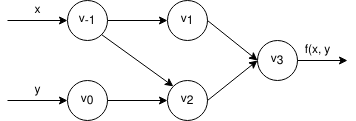
\includegraphics[scale=0.6]{./assets/function_trace.png}
  \caption{Computational graph of $f(x, y) = x^2 + (x - y)$}
  \label{fig:func_trace}
\end{figure}

\begin{table}
  \begin{center}
    \begin{tabular}{ l l l l l | l l l l l }
      \hline
      \multicolumn{5}{l}{Primal trace} & \multicolumn{5}{l}{Tangent trace} \\
      \hline
$v_{-1} $&$=$&$x$&$=$&$2$             &$v'_{-1}$&$=$&$x'$&$=$&$1$ \\
$v_0    $&$=$&$y$&$=$&$1$             &$v'_{0}$&$=$&$y'$&$=$&$0$ \\
      \hline
$v_1    $&$=$&$v_{-1}^2$&$=$&$4$      &$v'_{1}$&$=$&$2*v_{-1}$&$=$&$4$ \\
$v_2    $&$=$&$v_{-1} - v_{0}$&$=$&$1$&$v'_{2}$&$=$&$v'_{-1}-v'_{0}$&$=$&$1$ \\
$v_3    $&$=$&$v_1 + v_2$&$=$&$5$     &$v'_{3}$&$=$&$v'_1 + v'_2$&$=$&$5$ \\
      \hline
$f      $&$=$&$v_3$&$=$&$5$           &$f'$&$=$&$v'_3$&$=$&$5$ \\
      \hline
    \end{tabular}
  \end{center}
  \caption{Primal and tangent traces of $f(x, y) = x^2 + (x - y)$}
  \label{table:func_trace}
\end{table}
